% Algorithm

We implemented and analysed two additional algorithms in addition to the brute force algorithm that was required. One of them is the \emph{Knuth-Morris-Pratt} (KMP) algorithm with the other algorithm being \emph{Two-way String Matching}. All of the implementation was done in Python.

\section*{Brute Force Algorithm}
\begin{figure}[h!]
    \centering
    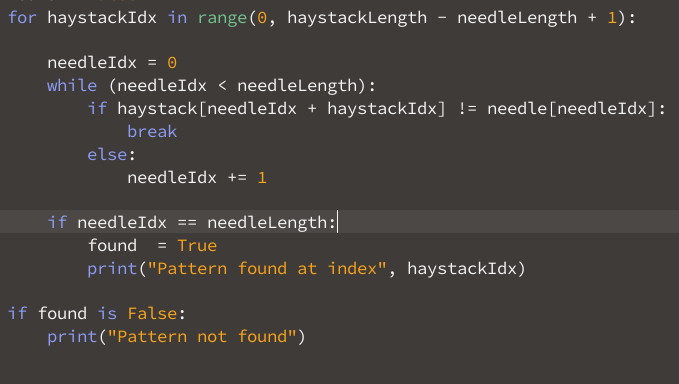
\includegraphics[width=0.50\textwidth]{images/brute_force.png}
    \caption{Code snippet of our brute force implementation}
\end{figure}

We first initialised a haystackId for the substring of the haystack that we are going to compare our needle with. This algorithm will begin by comparing the first letter of the needle with each letter of the substring, if they are the same, it will move on to the second letter and so on until the entire needle is traversed successfuly in which case, it is matched or the letters are no longer the same, which results in the \emph{if} case and hence, breaking. Then, the position of the substring will move by one character. 

Let $n, m$ be the length of the haystack and the needle respectively. For a complete search, we would need to go through all characters of the haystack. This means that we need to check $m - n + 1$ substrings. In the inner loop, we would need to compare each character of the needle to each character of the substring of the haystack. In the best case scenario, in the inner loop, the first character is never the same as the first character of the substring, i.e. the character doesn't exist in the haystack. This would just be $\mathcal{O}(1)$ in the inner loop. However, in the worst case, it would have to traverse through the entire length of the needle making the time complexity $\mathcal{O}O(m)$. Hence, this means that for this brute force algorithm, the best case time complexity is $\mathcal{O}(n - m + 1)$ while the worst case is $\mathcal{O}(n - m + 1)(m)$. This worst case scenario can be simplified to being $\mathcal{O}(mn)$ and the best case being $\mathcal{O}(n)$.

There is nothing to analyse for space complexity since we do not need to store any data.

\section*{KMP}

\begin{figure}[h]
    \centering
    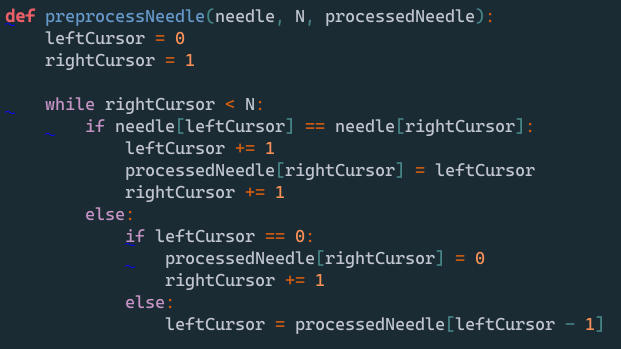
\includegraphics[width=0.50\textwidth]{images/preprocessKMP.png}
    \caption{Preprocess Function for KMP}
\end{figure}

In order to use the KMP Algorithm to search for our needle, we first needed to preprocess the substring. This is done so that we can calculate the values of how many characters we can skip comparing based on the point where the previous search ended. This is why there is an improvement in time complexity over the brute force algorithm where it compares every character in for every search. 

The function shown in Figure 2 has \emph{processedNeedle}, an array which stores the length of the longest prefix, suffix pairs. This tells us how many characters that do not need to be compared to one another in the next instance of a search when a mismatch happens in the current search. We calculate the value such that if the needle[leftCursor] and needle[rightCursor] matches, we increment leftCursor and assigns this value to the \emph{processedNeedle}. If there wasn't a match and the leftCursor is pointing to the first character, we reinitialise it. The point of all of this is to find characters which form both the prefix and suffix of the needle as we iterate through the needle.

\begin{figure}[h!]
    \centering
    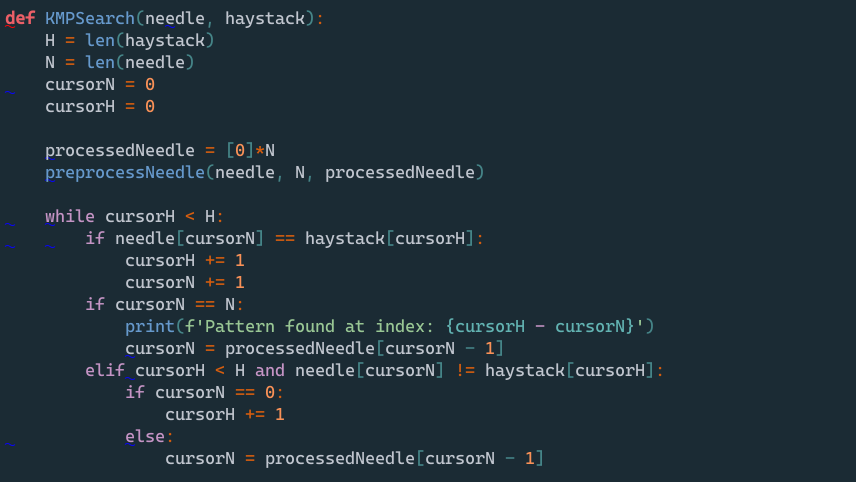
\includegraphics[width=0.50\textwidth]{images/KMP.png}
    \caption{KMP Search Function}
\end{figure}

After initialising the variables, we would need to preprocess the needle using the function in Fig 2. Since the length of the haystack and needle are $n, m$ respectively, we would begin comparison of the needle and the haystack and increment the value of the cursor while they keep matching. The \emph{if cursorN == N} indicates that all characters match with each other and the pattern is found. The benefit of KMP comes when there is a mismatch. If the mismatch happens at index $a$, this means that the first $a - 1$ characters of the needle matches with the first $a - 1$ characters of the haystack. From the preprocessing, we know that \emph{processedNeedle[a - 1]} is the number of characters that are both the prefix and suffix of that substring of the needle of length a. This means that we do not need to match the $a - 1$ characters because we know that these characters will match.

Since we do not need to do the comparison for those that are already matched, we only need to do one comparison for each character in the haystack. This means that the time complexity of the matching will be $\mathcal{O}(n)$. However, time is taken to do the preprocessing. Since we need to calculate the value of the prefix suffix pairs for each character in the needle, this would mean that the time complexity is $\mathcal{O}(m)$. Since the preprocessing and the matching happens linearly, we can say that the time complexity of the algorithm is $\mathcal{O}(n+m)$. In the problem that we are given, the best case and worst case time complexity for KMP would remain the same. This is because we want to find all occurences of the needle in the haystack. Hence, we would need to go through all the characters of the string even if a match is found in the first index. This means that the best case and worst case time complexity remains $\mathcal{O}(n+m)$.

The improvement to a linear time complexity in the worst case from $\mathcal{O}(mn)$ to $\mathcal{O}(m + n)$ comes with a tradeoff in space complexity. In the case of brute force, there is no need to store any data. However, the efficiency in KMP comes from the existence of the lookup table which is the array which tells us how many characters we do not need to match. The size of this array is equivalent to the length of the needle that we are searching for. Thus, the space complexity for KMP would be $\mathcal{O}(m)$.

\section*{Analysis}
\subsection*{Empirical Analysis}

\begin{figure}[h!]
    \centering
    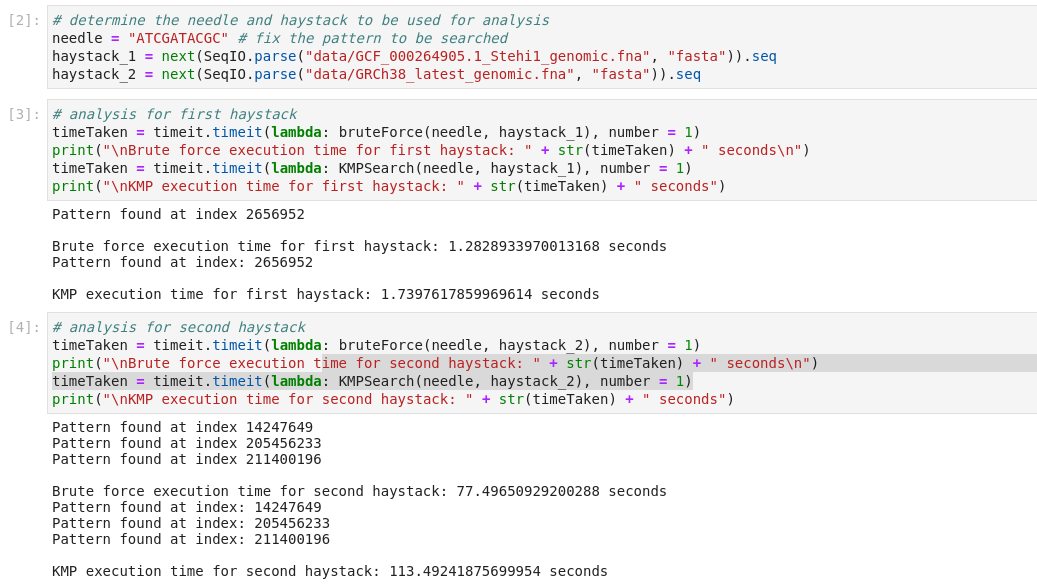
\includegraphics[width=0.50\textwidth]{images/jupyter.png}
    \caption{Timings}
\end{figure}

Based on the empirical analysis that we have done above, we can see that for most cases that we tested. Brute force actually take a shorter amount of time compared to KMP even though we have mentioned above that KMP should theoretically be faster since it's time complexity is $\mathcal{O}(n+m)$ in comparison to the worst case time complexity of Brute Force which is $\mathcal{O}(mn)$. However, this worst case scenario would occur only when the comparison for the substring is the same until the last character. For example, a needle of "AAAC" and a haystack filled completely with "A"s. However, this is not the case that we're dealing with in this problem and neither is this something that will reasonably happen in a real search. On average, the number of comparisons that would have to be done everytime the character shifts is much less than $m$. Hence, we can reasonably say that the time complexity of brute force on average is $\Theta(n)$. This is why it is faster than KMP in the experiment that we have done since the KMP algorithm would still have a time complexity of $\mathcal{O}(n+m)$ even in the best case.

\begin{figure}[h!]
    \centering
    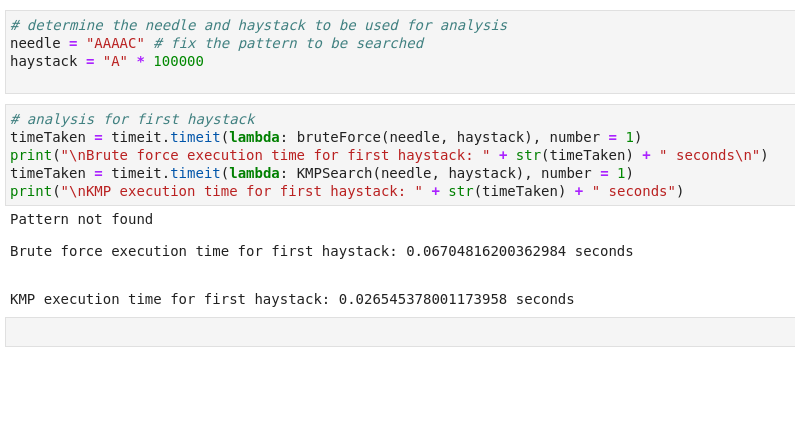
\includegraphics[width=0.50\textwidth]{images/worst_case.png}
    \caption{Timings}
\end{figure}

As has been mentioned, in this case, it is certainly faster for KMP than Brute Force to run. However, this is unrealistic since it is extremely improbable to encounter this in any string search scenario for a DNA